\documentclass[10pt,conference,onecolumn,compsoc]{IEEEtran}

\usepackage{rotating}
\usepackage{hyperref}
\usepackage{enumitem}
\setlist[itemize]{leftmargin=3 cm}
\setlist[enumerate]{leftmargin=3cm}

% *** CITATION PACKAGES ***
\ifCLASSOPTIONcompsoc
  \usepackage[nocompress]{cite}
\else
  \usepackage{cite}
\fi

% *** GRAPHICS RELATED PACKAGES ***
% \usepackage[pdftex]{graphicx}

% correct bad hyphenation here
\hyphenation{op-tical net-works semi-conduc-tor}


\begin{document}

\title{Leaping Llamas\\ for UTM CSCI 352 Spring 2017}

\author{Garrett Hay, Anderson Taylor, and Christina Hinton \\ % <-this % stops a space
}

\IEEEtitleabstractindextext{%
\begin{abstract}
We will be creating a similar game in the vein of Flappy Bird, which we are calling "Leaping Llamas." If the initial challenge proves to be trivial, we intend to add combat elements to increase the difficulty. Players looking for a casual yet challenging game should enjoy Leaping Llamas.
\end{abstract}
}
\maketitle

\IEEEdisplaynontitleabstractindextext
\IEEEpeerreviewmaketitle

\section{Introduction}
	The goal of this project is to create a simple yet fun game that can be played by anyone on a windows computer using only a mouse and keyboard.  For the type and content of the game we decided to go with a similar style to the popular game “Flappy Bird”.  At minimum we would like to include all of the basic functionality of the original game, so things like the auto generated level that is continuous and a high score system will definitely be incorporated into the app.
	
	Once all of the basic functionality described above is implemented we have plans to add additional functionality including variable difficulty settings and possibly even a “bullet hell” type game mode. We’re confident this will not only be an enjoyable experience for us the creators, but we also believe it will be fun for our peers to play post launch. By taking the “Flappy Bird” formula and making a more challenging experience, we think we can make a game that is relatively simple, but ultimately hard to master.
 

\subsection{Background}
	"Flappy Bird" is a game where the player controls a small bird, using inputs to lift the bird in order to navigate through pipes. Gravity pushes the bird down, but inputs can easily send the bird too high.

	If we reach our initial goals, we will convert Leaping Llamas into a bullet hell. A bullet hell is a game in which players must navigate through hordes of enemy projectiles without being hit. We believe it will make the game hilariously difficult and add an interesting twist to the Flappy Bird formula.

	We decided to tackle this project because it's a simple, universally-recognized game. It's known for being fun and addictive. We want to make a game that's cute, funny, and addicting, and a game like Flappy Bird is a fantastic inspiration to us.

\subsection{Challenges}
	We expect that insuring the player character's movement is smooth and responsive will be difficult. Hit boxes and fail states will be initially difficult. If we decide to have randomly generated pipes, we believe this will prove to be extremely tricky.

\section{Scope}
	Our main goal is to make Leaping Llamas, a simple Flappy Bird-like game. If we find ourselves finished well before the due date, we will add additional mechanics to further set it apart from Flappy Bird. Firstly, we would like to add extra llama images to be used or `skins'. Eventually bullet hell mechanics. Bullet hell mechanics are a usually extreme or hell-like amount of obstacles, usually bullet-like, that while challenging should be dodgable from somewhere on-screen.  Secondly, we would like to add onto the existing game in the form of animating objects, in order of: the background, the llama, any buttons, and any obstacles like 'pipes' and/or bullet-likes. 

\subsection{Requirements}
	As part of fleshing out the scope of your requirements, you'll also need to keep in mind both your functional and non-functional requirements.  These should be listed, and explained in detail as necessary.  Use this area to explain how you gathered these requirements.

\subsubsection{Functional}
	\begin{itemize}
	\item The game must be controlled with ``Spacebar'' key.
	\item The game must be implemented with C\# WPF.
	\item The game must feature music and sound effects.
	\item The game must feature obstacle generation with several different difficulty options.
	\item The game must be pausable with the ``P'' key.
	\item The game must end with the ``ESC'' key
	\end{itemize}

\subsubsection{Non-Functional}
	\begin{itemize}
	\item Performance -- Speed of obstacle generation.
	\item Scalability -- The obstacle generation will be potentially unlimited obstacle generation.
	\end{itemize}

\subsection{Use Cases}

%Case 1
\begin{itemize}
\item[Use Case Number:] 1
\item[Use Case Name:] Start Window
\item[Description:] The user on the program starts the program. The user will choose whether to start the game, see the high scores, change the difficulty, or exit the program.
\end{itemize}
\begin{enumerate}
\item The user shall press "Start" button.
\item[Termination Outcome:] The user will go to Case: 2.
\end{enumerate}
Alternative: User chooses the "Difficulty" button
\begin{enumerate}
\item The user shall press "Difficulty" button.
\item The program cycles through different difficulties.
\item[Termination Outcome:] The user will go to Case: 1.
\end{enumerate}
Alternative: User chooses the "High Score" button
\begin{enumerate}
\item The user shall press "High Score" button.
\item The program go to the High Score screen.
\item[Termination Outcome:] The user will go to Case: 4.
\end{enumerate}
Alternative: User chooses the "Exit" button
\begin{enumerate}
\item The user shall press "Exit" button.
\item The program will end.
\item[Termination Outcome:] The user has kill the program.
\end{enumerate}

%Case 2
\begin{itemize}
\item[Use Case Number:] 2
\item[Use Case Name:] Playing \textit{Leaping Llamas}
\item[Description:] The user on the program starts the game. The user will make the llama leap over and between the obstacles until the llama hits a obstacle. This will send the user to the scoreboard.
\end{itemize}

\begin{enumerate}
\item The user shall press "Spacebar" button to "Leap" over obstacles.
\item The game will count up by 1 for each obstacle on its counter.
\item The game will end once the user's Llama hits an obstacle
\item[Termination Outcome:] The user has played the game portion of the program.
\end{enumerate}


%Case 3
\begin{itemize}
\item[Use Case Number:] 3
\item[Use Case Name:] Scoreboard after 'Game Over'
\item[Description:] A shopper on our site has finished shopping.  They will click on a ``Checkout" button.  This will kick off a process to calculate cart total, any taxes, shipping rates, and collect payment from the shopper.

\end{itemize}

\begin{enumerate}
\item The program shall open a window with the user's score and a "Retry" and "Next" buttons.
\item The user shall select "Retry" button and proceed back to Use Case: 1 until selecting the "Next" button.
\item[Termination Outcome:] The user will either replay the game with new score or proceed to the High Score screen.
\end{enumerate}

Alternative: The user scored a High Score
\begin{enumerate}
\item The program shall open a window with a text box and shall prompt the user for a username and a "Retry" and "Next" buttons.
\item The username shall be stored along with the user's score to a file with other High scores.
\item The user shall select "Retry" button and proceed back to Use Case: 1 until selecting the "Next" button.
\item[Termination Outcome:] The user will either replay the game with new score or proceed to the High Score screen.
\end{enumerate}


%Case 4
\begin{itemize}
\item[Use Case Number:] 4
\item[Use Case Name:] High Score screen
\item[Description:] A user has finished playing. The user will be shown the top 10 High Scores on the game. They will choose either to play again or return to the title screen.

\end{itemize}

\begin{enumerate}
\item The window shall display the High scores in nonincreasing order from the top of the window.
\item The user shall choose whether to click the "Retry" button.
\item The program will return to the game on the same difficulty.
\item[Termination Outcome:] The user will either replay the game with new score.
\end{enumerate}

Alternative: The user chooses the "Title" button
\begin{enumerate}
\item The window shall display the High scores in nonincreasing order from the top of the window.
\item The user shall choose whether to click the "Title" button.
\item The program will return to the title screen.
\item[Termination Outcome:] The user will be at the Title screen at case: 1. 
\end{enumerate}

\begin{center}
\begin{figure}[ht!]
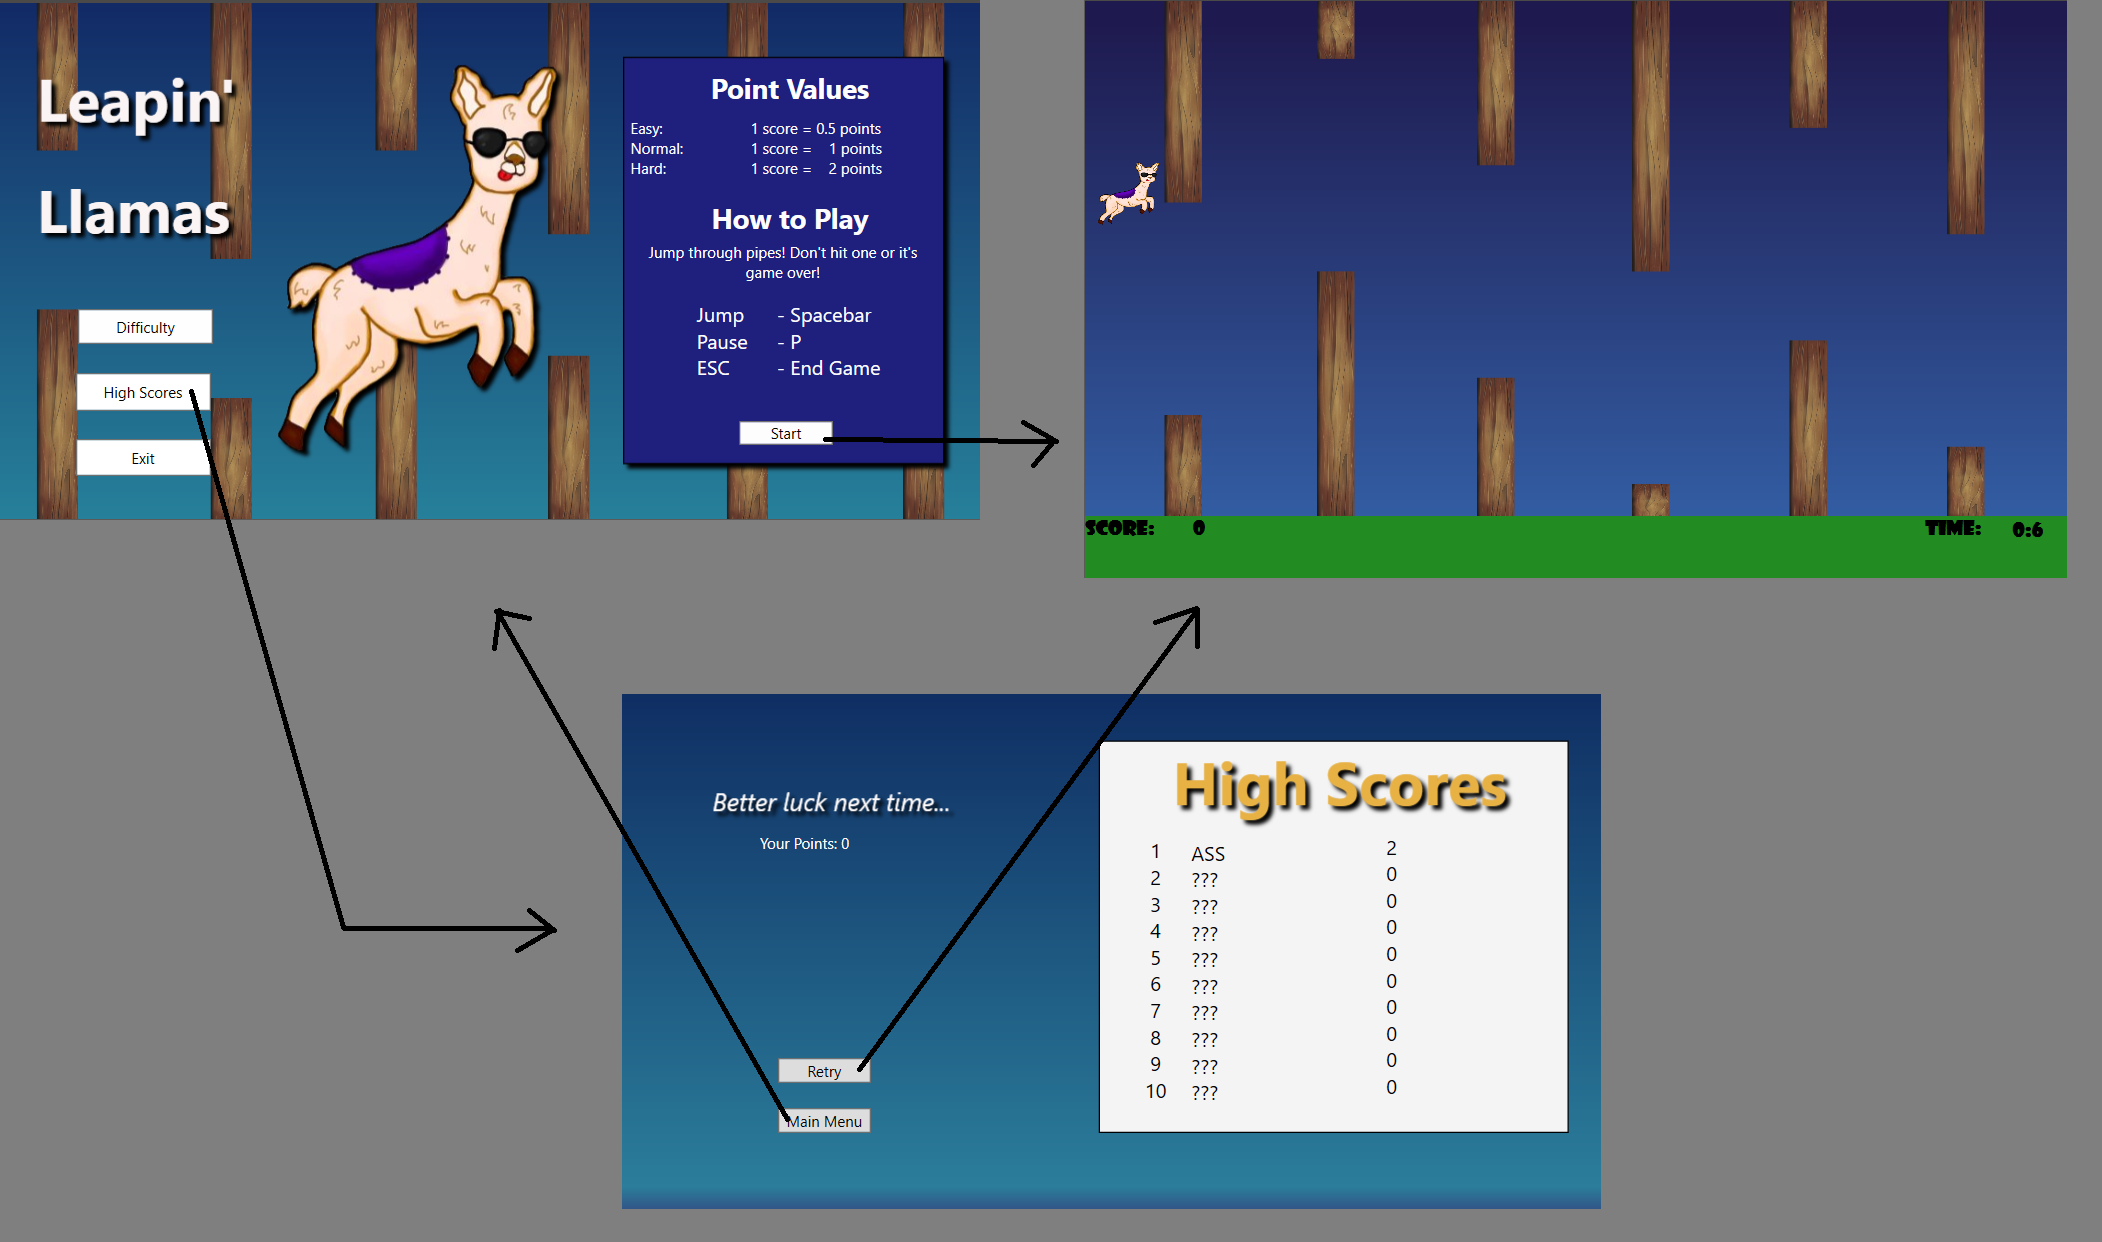
\includegraphics[scale = 0.4]{Mockup.png}
\caption{First picture, This is full number of Mock-Interfaces made.}
\label{fig:mockup}
\end{figure}
\end{center}


\subsection{Interface Mockups}
For all below see Figure \ref{fig:mockup}
First in order, the user will begin on the `Title' screen, optionally choose from the changing difficulty button or leave it to default to `normal' choose one of the button to move to the corresponding screen. Next the `Game' screen will always lead to the `Score' screen at the end of the game. The `Score' screen has at least two choices. First, to retry and return to the `Game' screen or second to exit to the `Title' screen. Another choice may appear if the player has earned enough point to join the Highscore board and can enter a nickname up to nine characters in length before choosing one of the previous choices.

\section{Project Timeline}
See Figure \ref{fig:timeline} below.
\begin{figure}[ht!]
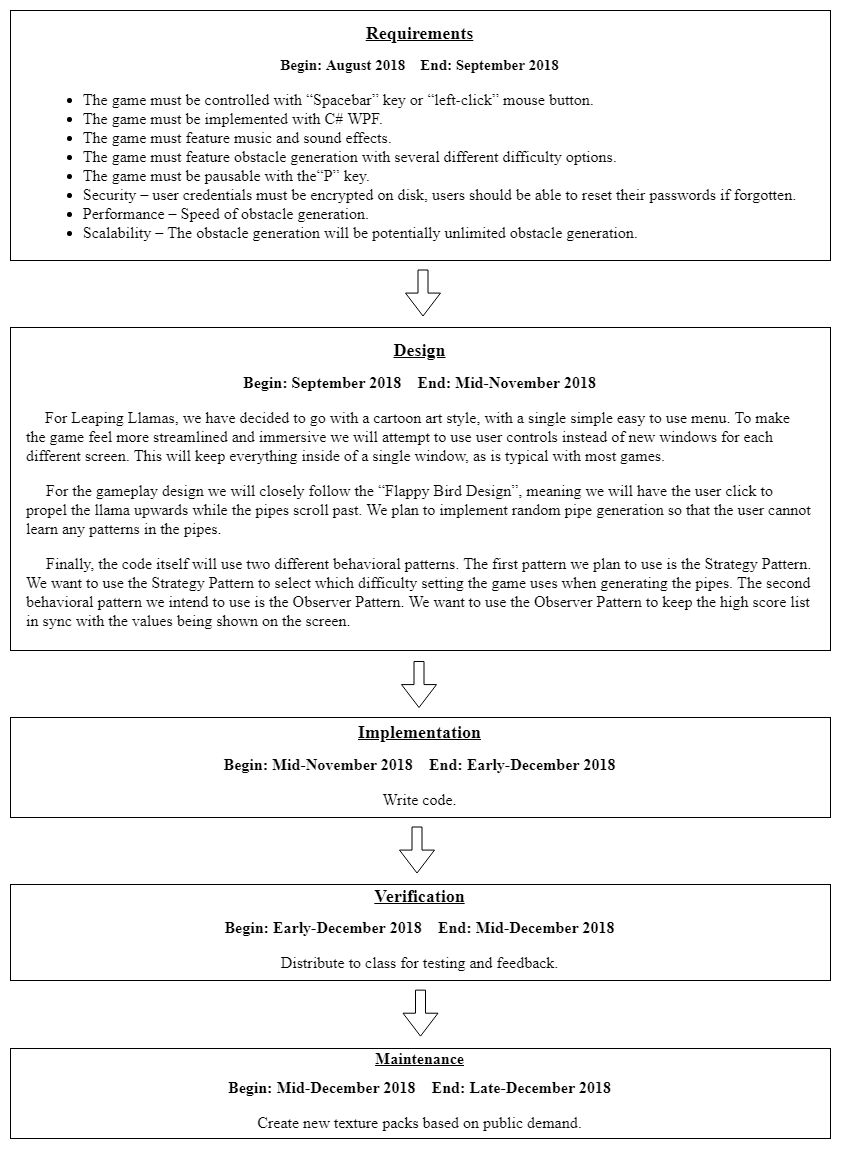
\includegraphics[scale=0.5]{ProposalTimeline.png}
\caption{Proposed timeline, This is a rough estimate of the project timeline.}
\label{fig:timeline}
\end{figure}

\section{Project Structure}
We choose to make the difficulty button change to the current difficulty upon clicking it. We also choose to make the new highscore option invisible unless the amount of points earned is reached.
As for the game portion we made the `esc' and `p' keys shortcuts to ending the game instantly and pausing the game respectfully. We also made the portion of the screen above the main screen inaccessible.

\subsection{UML Outline}
See Figure \ref{dia}.

\begin{sidewaysfigure}[!ht]
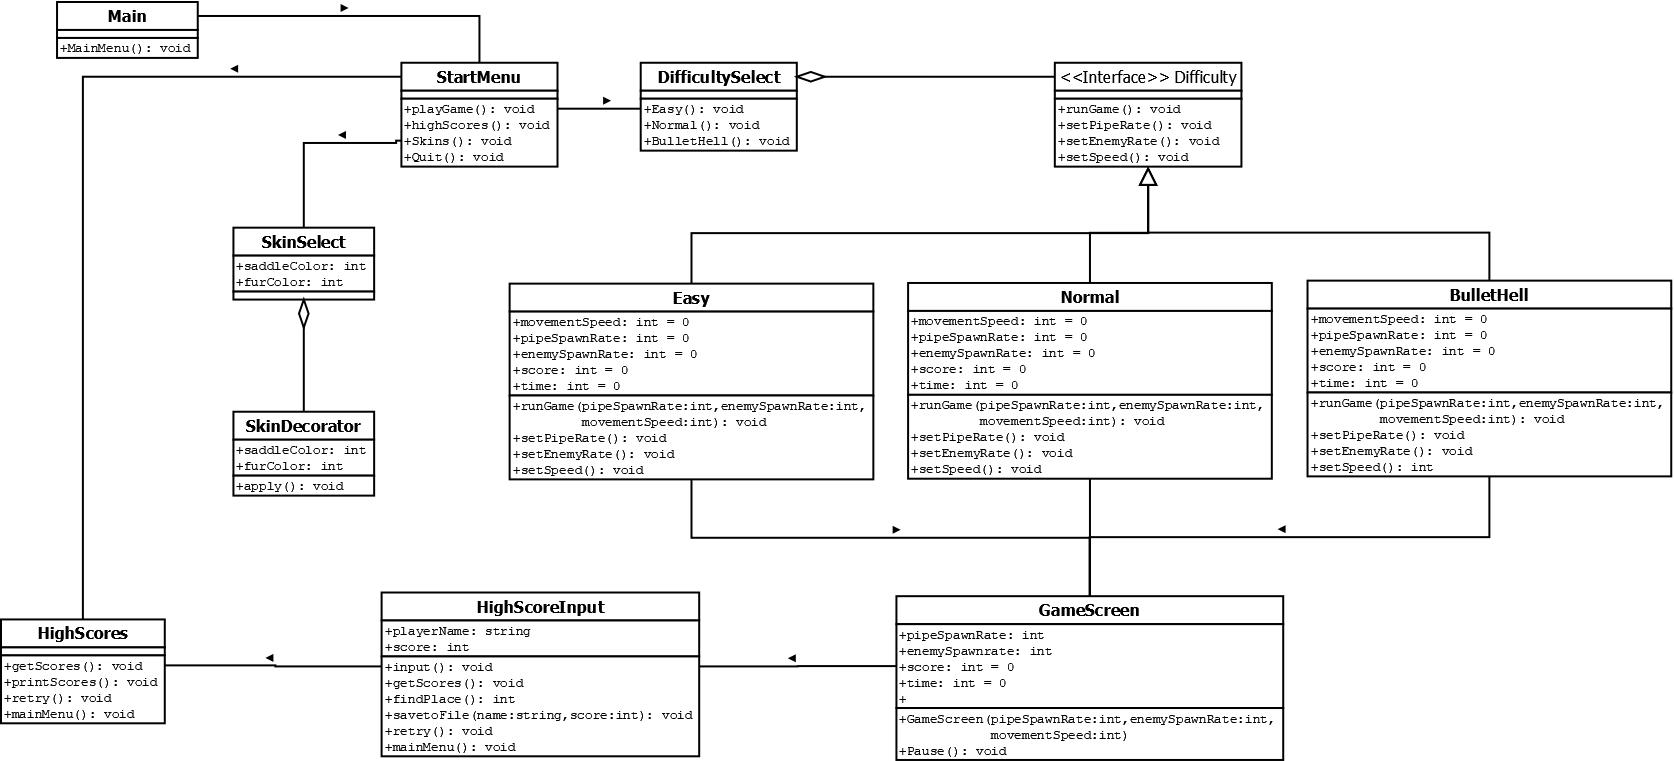
\includegraphics[scale=0.3]{LeapingLlamas.png}
\caption{diagram of project using the Decorator Pattern and Strategy Pattern.}
\label{dia}
\end{sidewaysfigure}

\subsection{Design Patterns Used}
Our Program will be using 2 design patterns. The first is a Decorator Pattern for selecting different skins of llama. The second is a Strategy Pattern on the different difficulties we have different fence classes for.

\section{Results}
Leaping Llamas started to really take shape by deliverable 5. Previously, the project was mostly conceptual in nature, however between deliverables 4 and 5 the program really took shape and is a playable, interesting user experience. As the game stands now there are options for 3 different difficulties, a "infinitely" generated level that keeps high scores, and hit detection if the llama hits a barrier.

\subsection{Future Work}
Before the final submission we will implement different skins for the llama that the user can choose from. Aside from this the only thing we want to get fixed is the hitbox detection near the rear of the character. As for the far future plans for the project each member of our team will add the final version of the game to their Github.com accounts to showcase to potential employers.

\begin{thebibliography}{1}

\bibitem{IEEEhowto:kopka}
H.~Kopka and P.~W. Daly, \emph{A Guide to \LaTeX}, 3rd~ed.\hskip 1em plus
  0.5em minus 0.4em\relax Harlow, England: Addison-Wesley, 1999.

\end{thebibliography}

\begin{IEEEbiography}{Michael Shell}
Biography text here.
\end{IEEEbiography}

\begin{IEEEbiographynophoto}{John Doe}
Biography text here.
\end{IEEEbiographynophoto}

\begin{IEEEbiographynophoto}{Jane Doe}
Biography text here.
\end{IEEEbiographynophoto}
\end{document}


